\begin{figure}
\centering
\begin{tabular}{c|cccc}
\hline
Query & \#1 & \#2 & \#3 & \#4 \\
\hline
\\
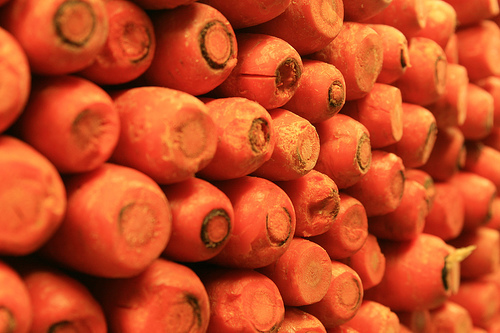
\includegraphics[width=0.16\linewidth,valign=c]{figs/neighbors/924.jpg} &
\includegraphics[width=0.16\linewidth,valign=c]{{figs/neighbors/924.jpg.neighbor_1}.JPEG} &
\includegraphics[width=0.16\linewidth,valign=c]{{figs/neighbors/924.jpg.neighbor_2}.JPEG} &
\includegraphics[width=0.16\linewidth,valign=c]{{figs/neighbors/924.jpg.neighbor_3}.JPEG} &
\includegraphics[width=0.16\linewidth,valign=c]{{figs/neighbors/924.jpg.neighbor_4}.JPEG} \\
\\
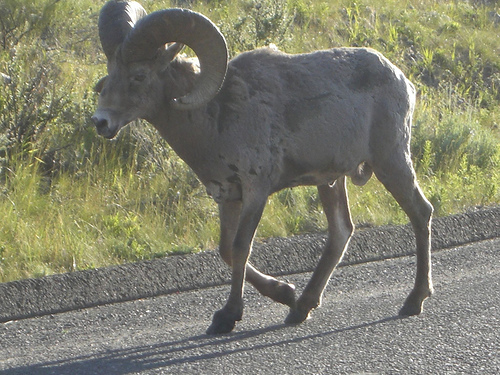
\includegraphics[width=0.16\linewidth,valign=c]{figs/neighbors/121.jpg} &
\includegraphics[width=0.16\linewidth,valign=c]{{figs/neighbors/121.jpg.neighbor_1}.JPEG} &
\iffalse
skip neighbor_2 -- duplicate of neighbor_1
\fi
\includegraphics[width=0.16\linewidth,valign=c]{{figs/neighbors/121.jpg.neighbor_3}.JPEG} &
\includegraphics[width=0.16\linewidth,valign=c]{{figs/neighbors/121.jpg.neighbor_4}.JPEG} &
\includegraphics[width=0.16\linewidth,valign=c]{{figs/neighbors/121.jpg.neighbor_5}.JPEG} \\
\\
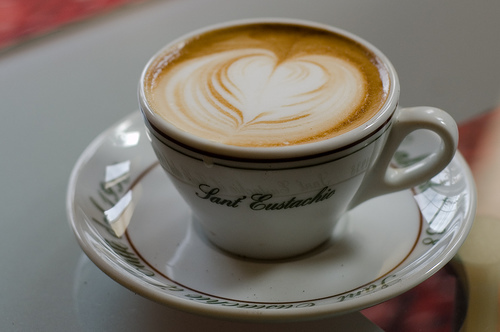
\includegraphics[width=0.16\linewidth,valign=c]{figs/neighbors/231.jpg} &
\includegraphics[width=0.16\linewidth,valign=c]{{figs/neighbors/231.jpg.neighbor_1}.JPEG} &
\includegraphics[width=0.16\linewidth,valign=c]{{figs/neighbors/231.jpg.neighbor_2}.JPEG} &
\includegraphics[width=0.16\linewidth,valign=c]{{figs/neighbors/231.jpg.neighbor_3}.JPEG} &
\includegraphics[width=0.16\linewidth,valign=c]{{figs/neighbors/231.jpg.neighbor_4}.JPEG} \\
\\
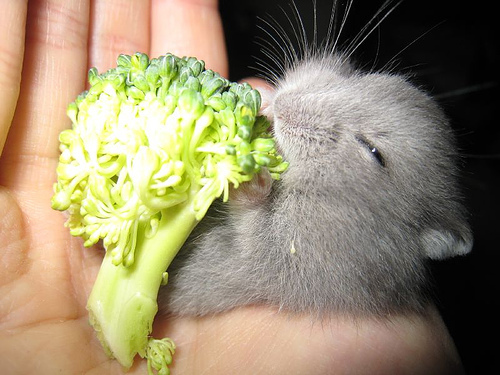
\includegraphics[width=0.16\linewidth,valign=c]{figs/neighbors/605.jpg} &
\includegraphics[width=0.16\linewidth,valign=c]{{figs/neighbors/605.jpg.neighbor_1}.JPEG} &
\includegraphics[width=0.16\linewidth,valign=c]{{figs/neighbors/605.jpg.neighbor_2}.JPEG} &
\includegraphics[width=0.16\linewidth,valign=c]{{figs/neighbors/605.jpg.neighbor_3}.JPEG} &
\includegraphics[width=0.16\linewidth,valign=c]{{figs/neighbors/605.jpg.neighbor_4}.JPEG} \\
\\
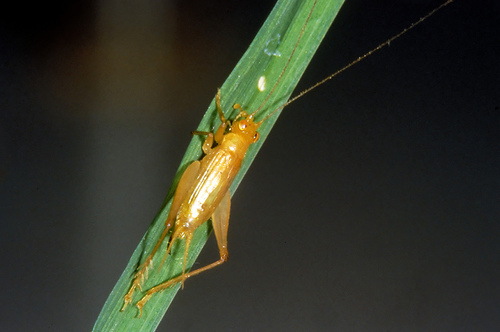
\includegraphics[width=0.16\linewidth,valign=c]{figs/neighbors/88.jpg} &
\includegraphics[width=0.16\linewidth,valign=c]{{figs/neighbors/88.jpg.neighbor_1}.JPEG} &
\includegraphics[width=0.16\linewidth,valign=c]{{figs/neighbors/88.jpg.neighbor_2}.JPEG} &
\includegraphics[width=0.16\linewidth,valign=c]{{figs/neighbors/88.jpg.neighbor_3}.JPEG} &
\includegraphics[width=0.16\linewidth,valign=c]{{figs/neighbors/88.jpg.neighbor_4}.JPEG} \\
\\
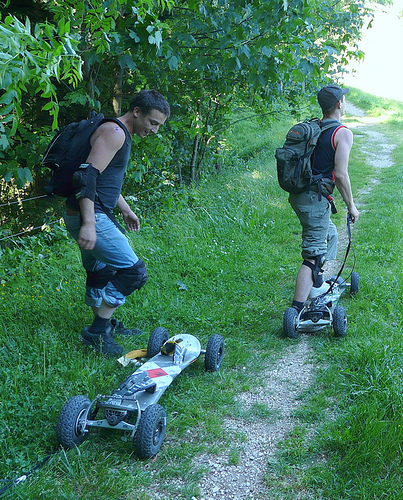
\includegraphics[width=0.16\linewidth,valign=c]{figs/neighbors/132.jpg} &
\includegraphics[width=0.16\linewidth,valign=c]{{figs/neighbors/132.jpg.neighbor_1}.JPEG} &
\includegraphics[width=0.16\linewidth,valign=c]{{figs/neighbors/132.jpg.neighbor_2}.JPEG} &
\includegraphics[width=0.16\linewidth,valign=c]{{figs/neighbors/132.jpg.neighbor_3}.JPEG} &
\includegraphics[width=0.16\linewidth,valign=c]{{figs/neighbors/132.jpg.neighbor_4}.JPEG} \\
\hline
\end{tabular}
\caption{
For the query images used in~\citet{datadep} (left),
nearest neighbors (by minimum cosine distance) from the ImageNet LSVRC~\citep{imagenet} training set in the \textit{fc6} feature space of the ImageNet-trained BiGAN encoder $E$.
(The \textit{fc6} weights are set randomly; this space is a random projection of the learned \textit{conv5} feature space.)
}
\lblfig{imagenetneighbors}
\end{figure}
